\section{Linguaggi utilizzati}

Si è deciso di utilizzare il metodo MVC (Model View Controller) per semplificare la gestione
e diminuire la ridondanza del codice.

\subsection{HTML5}
Il gruppo ha utilizzato il linguaggio di markup \textit{HTML5} per la
modellazione delle pagine web.

\subsection{PHP}
Il lato server è stato sviluppato utilizzando il linguaggio di programmazione \textit{PHP}

\subsection{SQL}
\textit{SQL} è stato utilizzato nella crazione del database, il quale è formato dalle seguenti tabelle:

\begin{itemize}
	\item \textit{Brand}: si riferisce alla marca del dispositivo;
	\item \textit{Model}: contiene le informazioni del modello di una marca;
	\item \textit{Purchase item}: contiene informazioni relative agli acquisti, dispositivi venduti e non;
	\item \textit{Repair item}: contiene informazioni relative alle riparazioni, comprese le riparazioni effettuate e non;
	\item \textit{sell item}: TODO;
	\item \textit{User}: contiene informazioni degli utenti;
\end{itemize}

Le tabelle \textit{Brand} e \textit{Model} sono già riempite con dataset; invece le tabelle \textit{Purchase item} e \textit{Repair item}
verranno riempite man mano che gli utenti eseguono le richieste.

\begin{figure}[H]
	\centering
	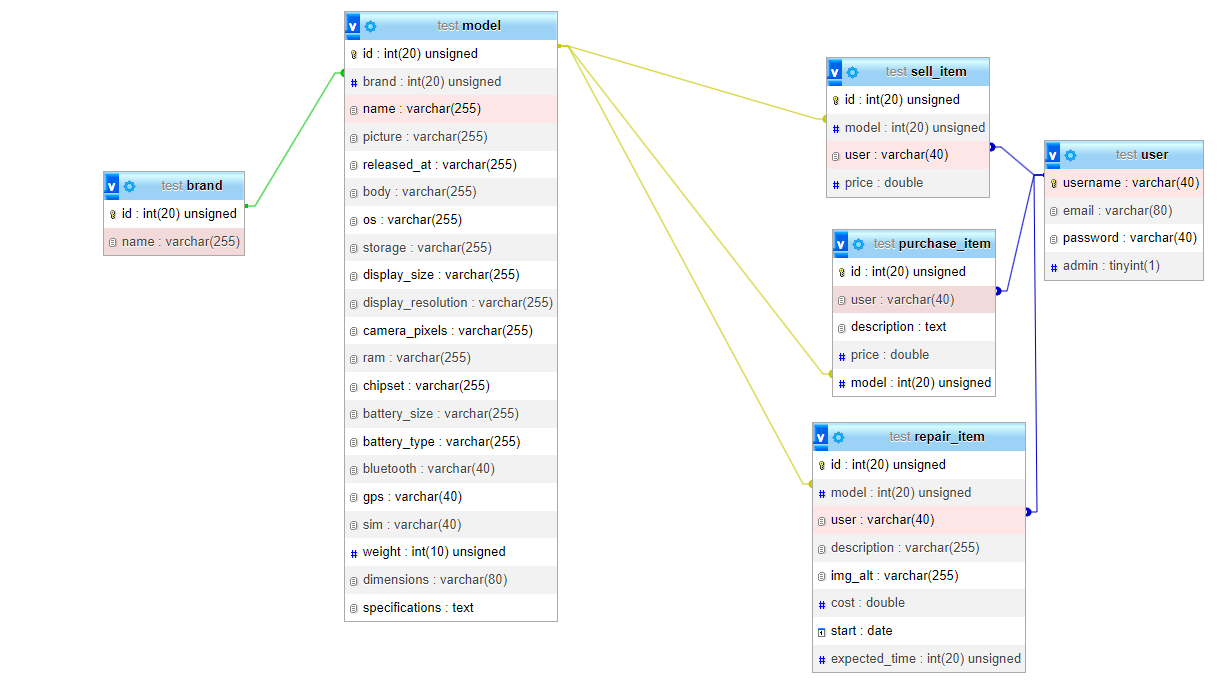
\includegraphics[scale=0.4]{res/database.png}
	\caption{Modello del database}
\end{figure}

\subsection{JavaScript}
\textit{JavaScript } è stato utilizzato per rendere il sito pi`u dinamico e migliorare l’esperienza utente. Occorre
precisare però che la sua disabilitazione o il suo mancato funzionamento non comportano in alcun
modo l’impossibilit`a di fruire dei servizi offerti dal sito.

Innazitutto viene utilizzato per applicazione di una rappresentazione di una serie di immagini, visualizzandole
una alla volta attraverso due pulsanti \textit{precedente} e \textit{successivo}; si può trovare un esempio d'uso
nella pagina principale.

Un suo secondo utilizzo è rendere visibile un pulsante a freccia in su che ha il compito di riportare l'utente
in cima alla pagina. Il punsante ovviamente diventa visibile e cliccabile quando l'utente ha scrollato(SI PUO DIRE?) la pagina in giu'

Infine viene utilizzato per controllare gli input tipo per Login e Registrazione, dove neccessitano di un controllo del formato
del testo inserito; in caso del formato sbagliato verrà visualizzata un suggerimento sotto al box di inserimento sul formato del
testo accettato